We define a control region enriched in top and $WW$ events to validate our method to estimate those backgrounds
with opposite flavor dilepton events. The selection criteria are the following:
\begin{itemize}
\item $|m_{\ell\ell} - m_Z| > 15\:\GeVcc$,
\item $M_T > 150\:\GeVcc$,
\item MET $>$ threshold for the $m_H=250\:\GeVcc$ selection,
\item $\Delta\phi\left(\mbox{jet},\mbox{MET}\right) >$ threshold for the $m_H=250\:\GeVcc$ selection. 
\end{itemize} 


%%%%%%%%
\begin{figure}[!hbtp]
\begin{center}
\subfigure[Muon channel]{\label{subfig:topww_mass_mm}
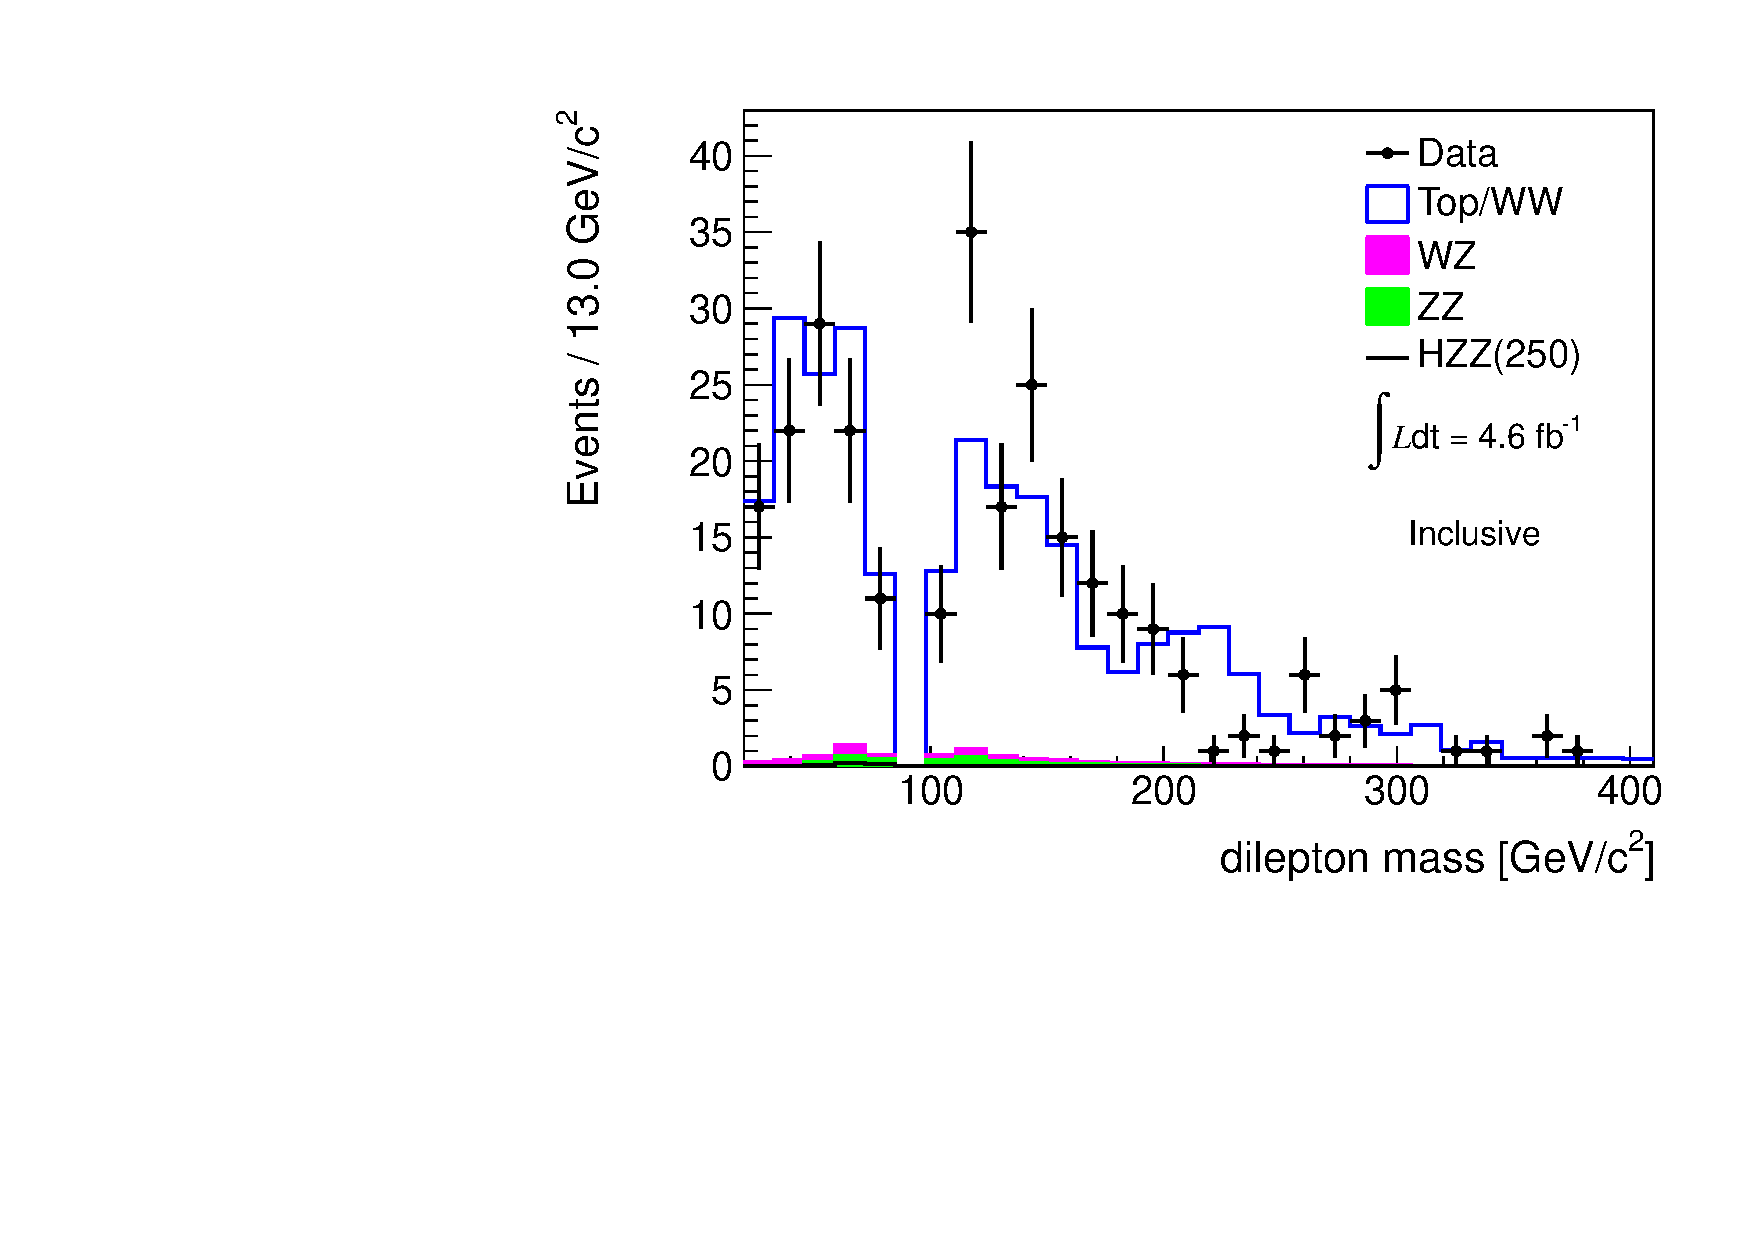
\includegraphics[width=.4\textwidth]{figures/topww_mH250_mm_mass_incl.pdf}}
\subfigure[Electron channel]{\label{subfig:topww_mass_ee}
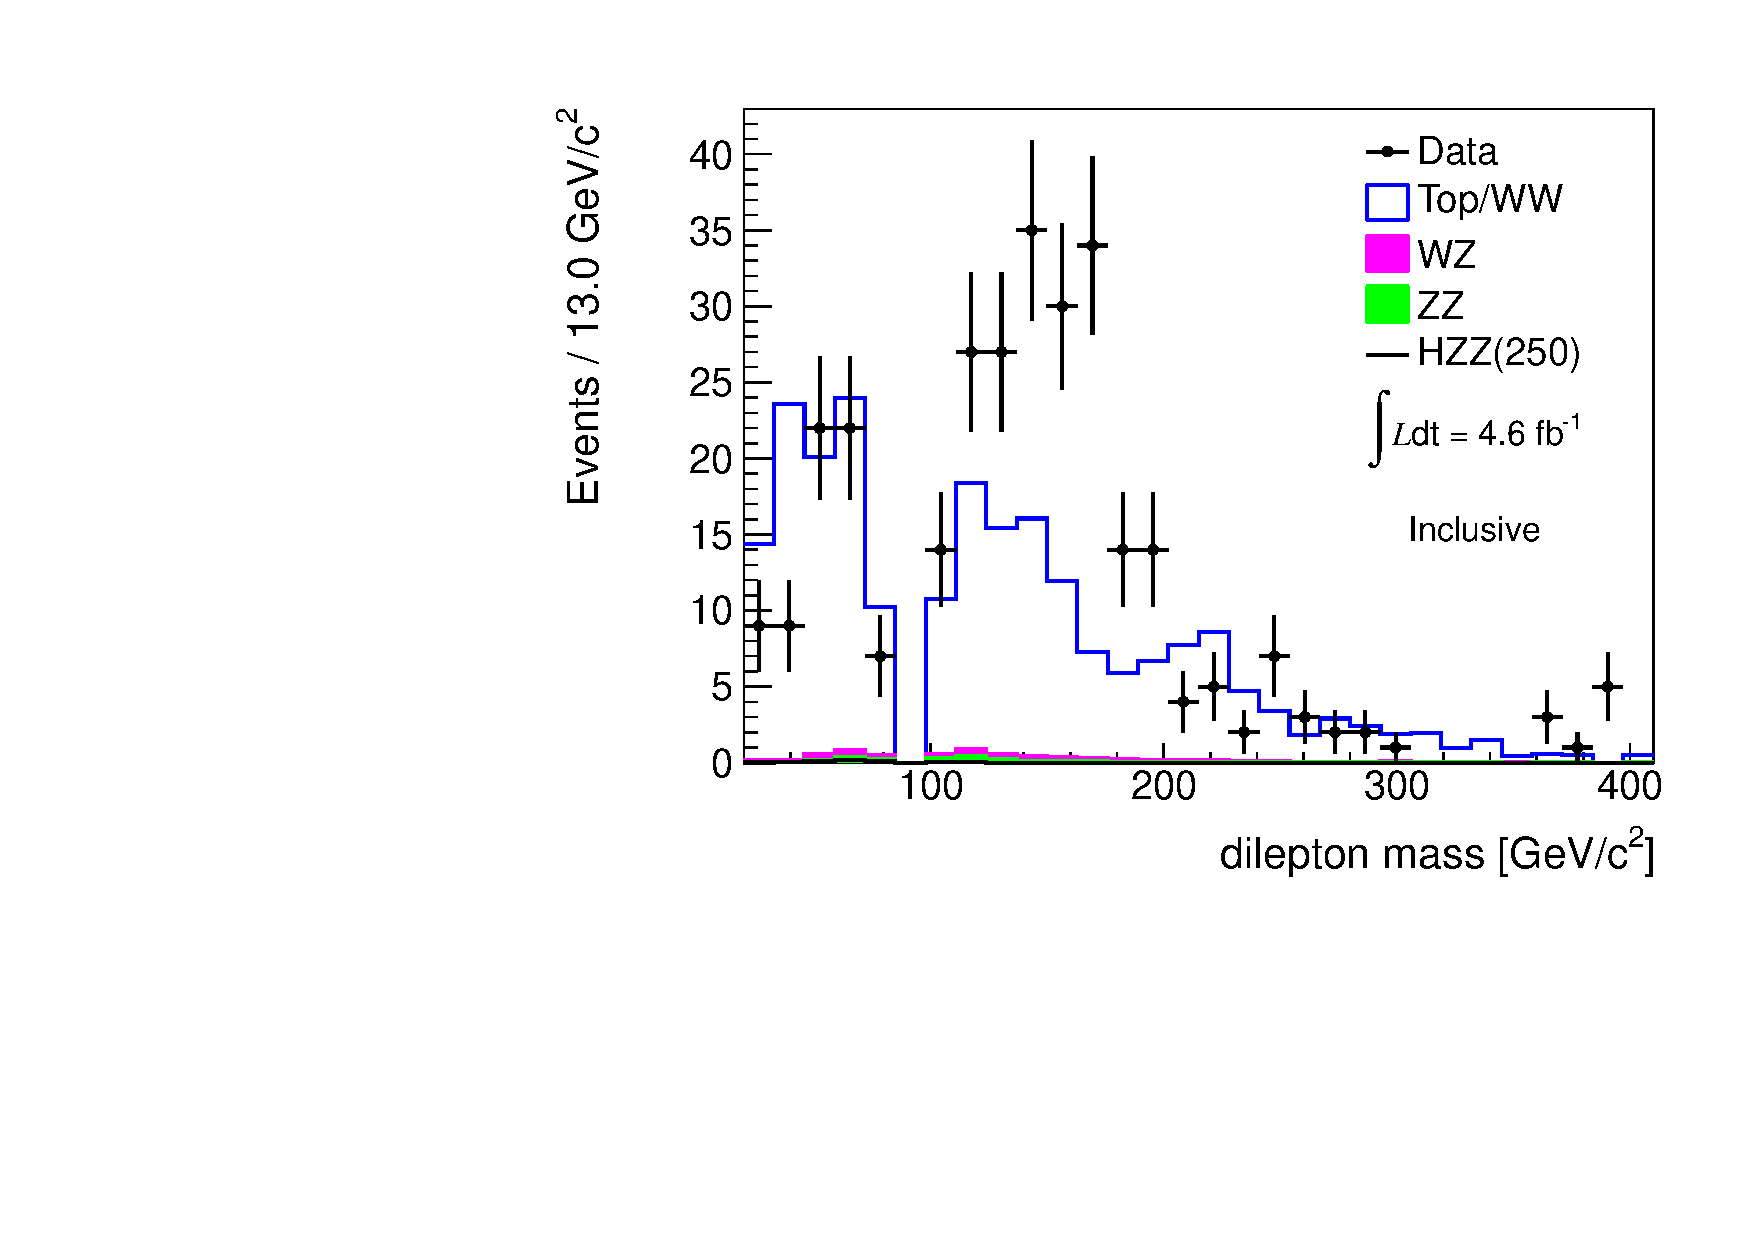
\includegraphics[width=.4\textwidth]{figures/topww_mH250_ee_mass_incl.pdf}}
\caption{Distribution for the dilepton mass in the top/$WW$ control region corresponding 
to $4.0$~\ifb of data in the muon~\subref{subfig:npv_mm} and electron~\subref{subfig:npv_ee} channels, 
compared to the expected from simulation for signal and background. The MC backgrounds are scaled as 
appropriate and the opposite flavor dilepton estimate of the top and $WW$ background is added to the stack.}
\label{fig:topww_mass}
\end{center}
\end{figure}
%%%%%%%%

%%%%%%%%
\begin{figure}[!hbtp]
\begin{center}
\subfigure[Muon channel]{\label{subfig:topww_dileppt_mm}
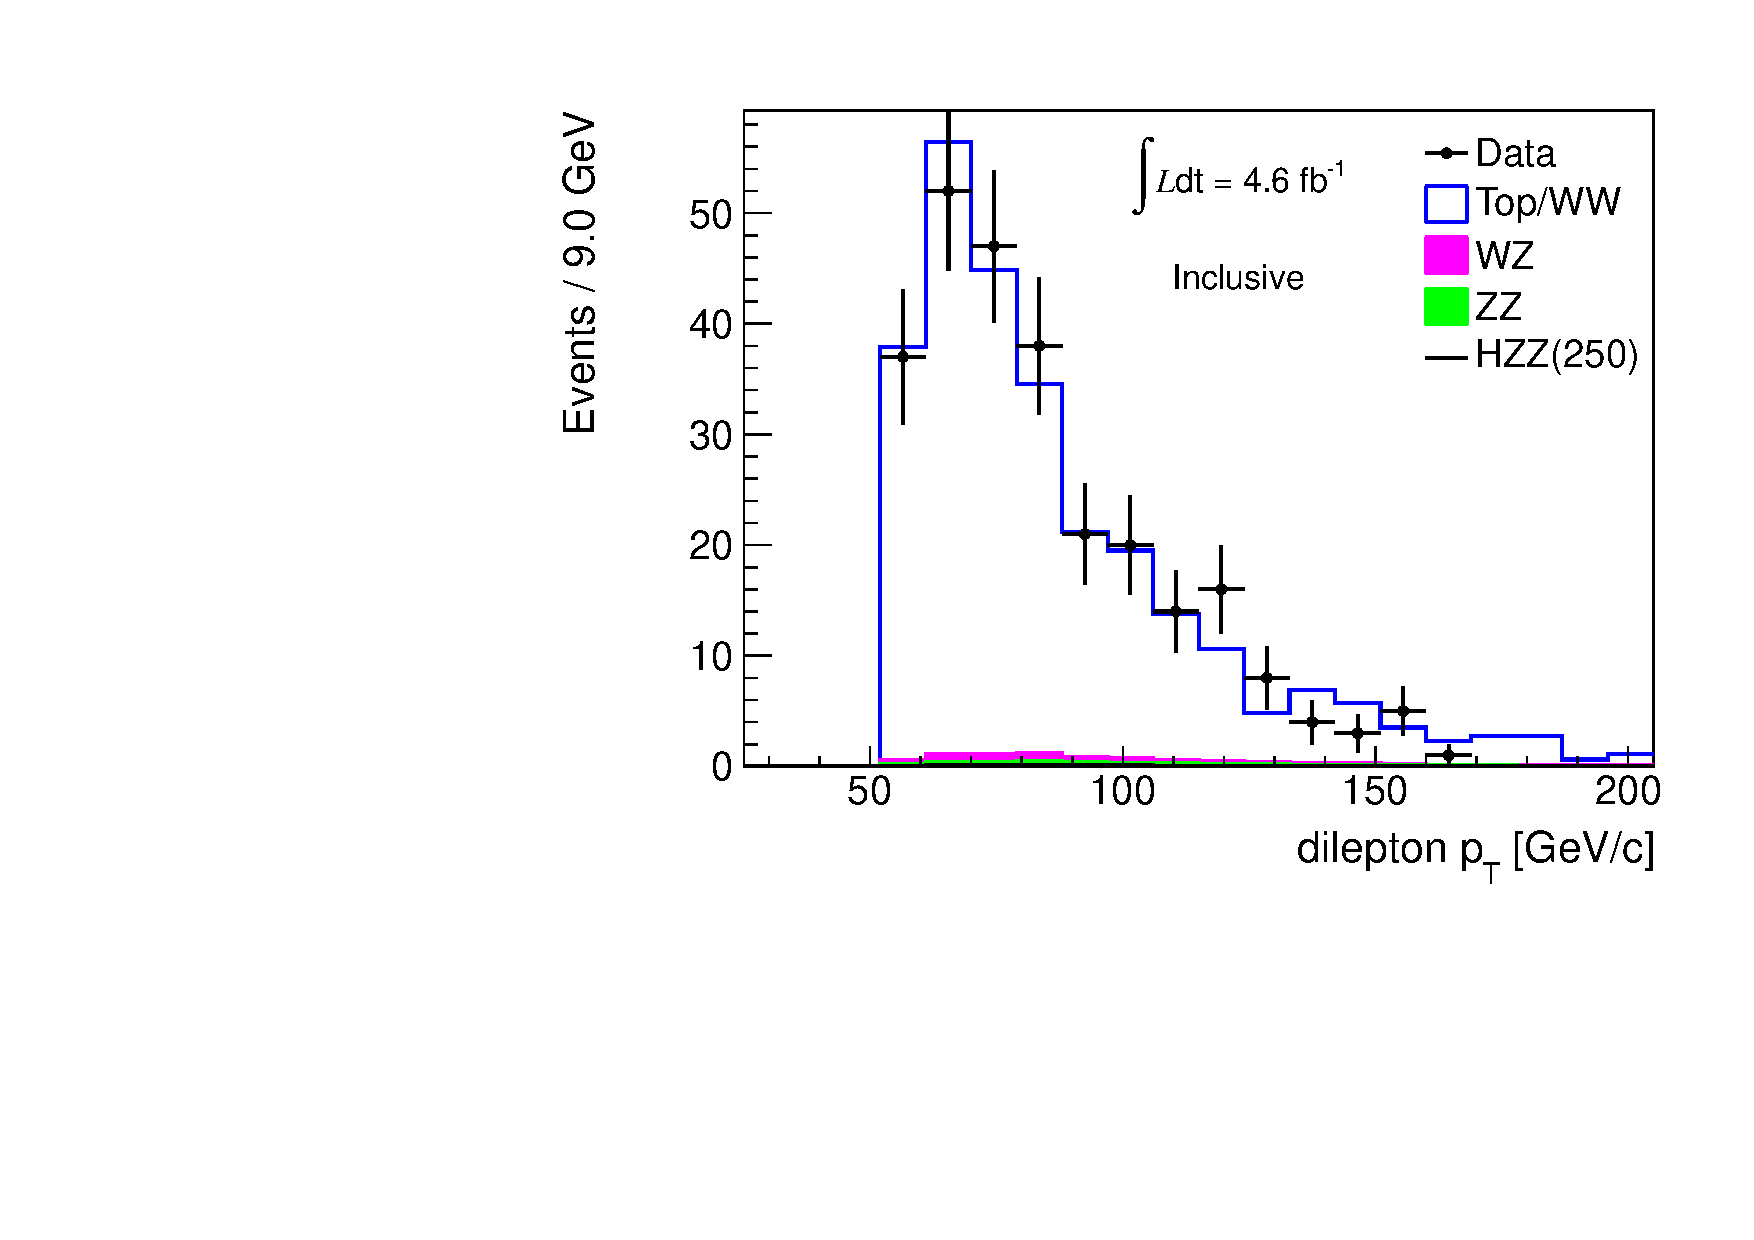
\includegraphics[width=.4\textwidth]{figures/topww_mH250_mm_dileppt_incl.pdf}}
\subfigure[Electron channel]{\label{subfig:topww_dileppt_ee}
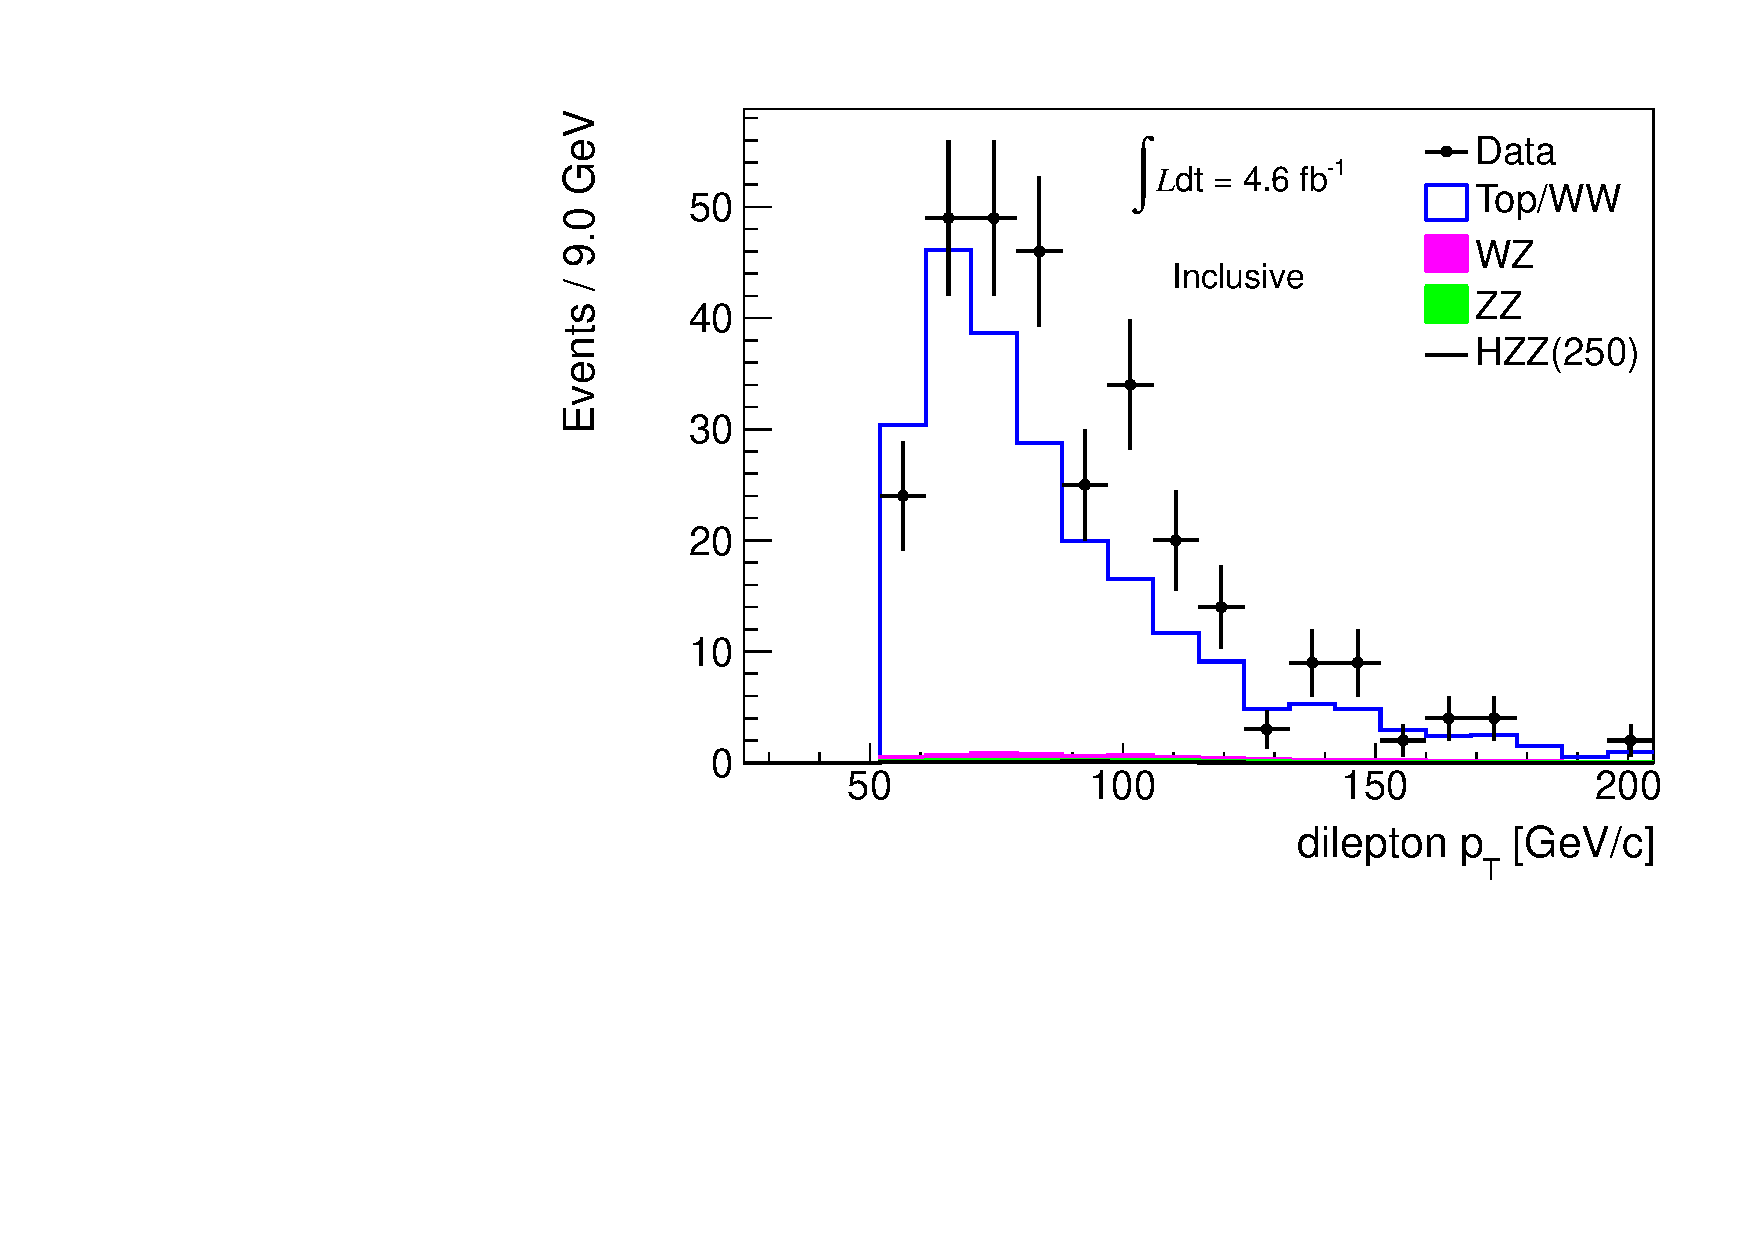
\includegraphics[width=.4\textwidth]{figures/topww_mH250_ee_dileppt_incl.pdf}}
\caption{Distribution for the dilepton $p_T$ in the top/$WW$ control region corresponding 
to $4.0$~\ifb of data in the muon~\subref{subfig:npv_mm} and electron~\subref{subfig:npv_ee} channels, 
compared to the expected from simulation for signal and background. The MC backgrounds are scaled as 
appropriate and the opposite flavor dilepton estimate of the top and $WW$ background is added to the stack.}
\label{fig:topww_dileppt}
\end{center}
\end{figure}
%%%%%%%%

%%%%%%%%
\begin{figure}[!hbtp]
\begin{center}
\subfigure[Muon channel]{\label{subfig:topww_metlog_mm}
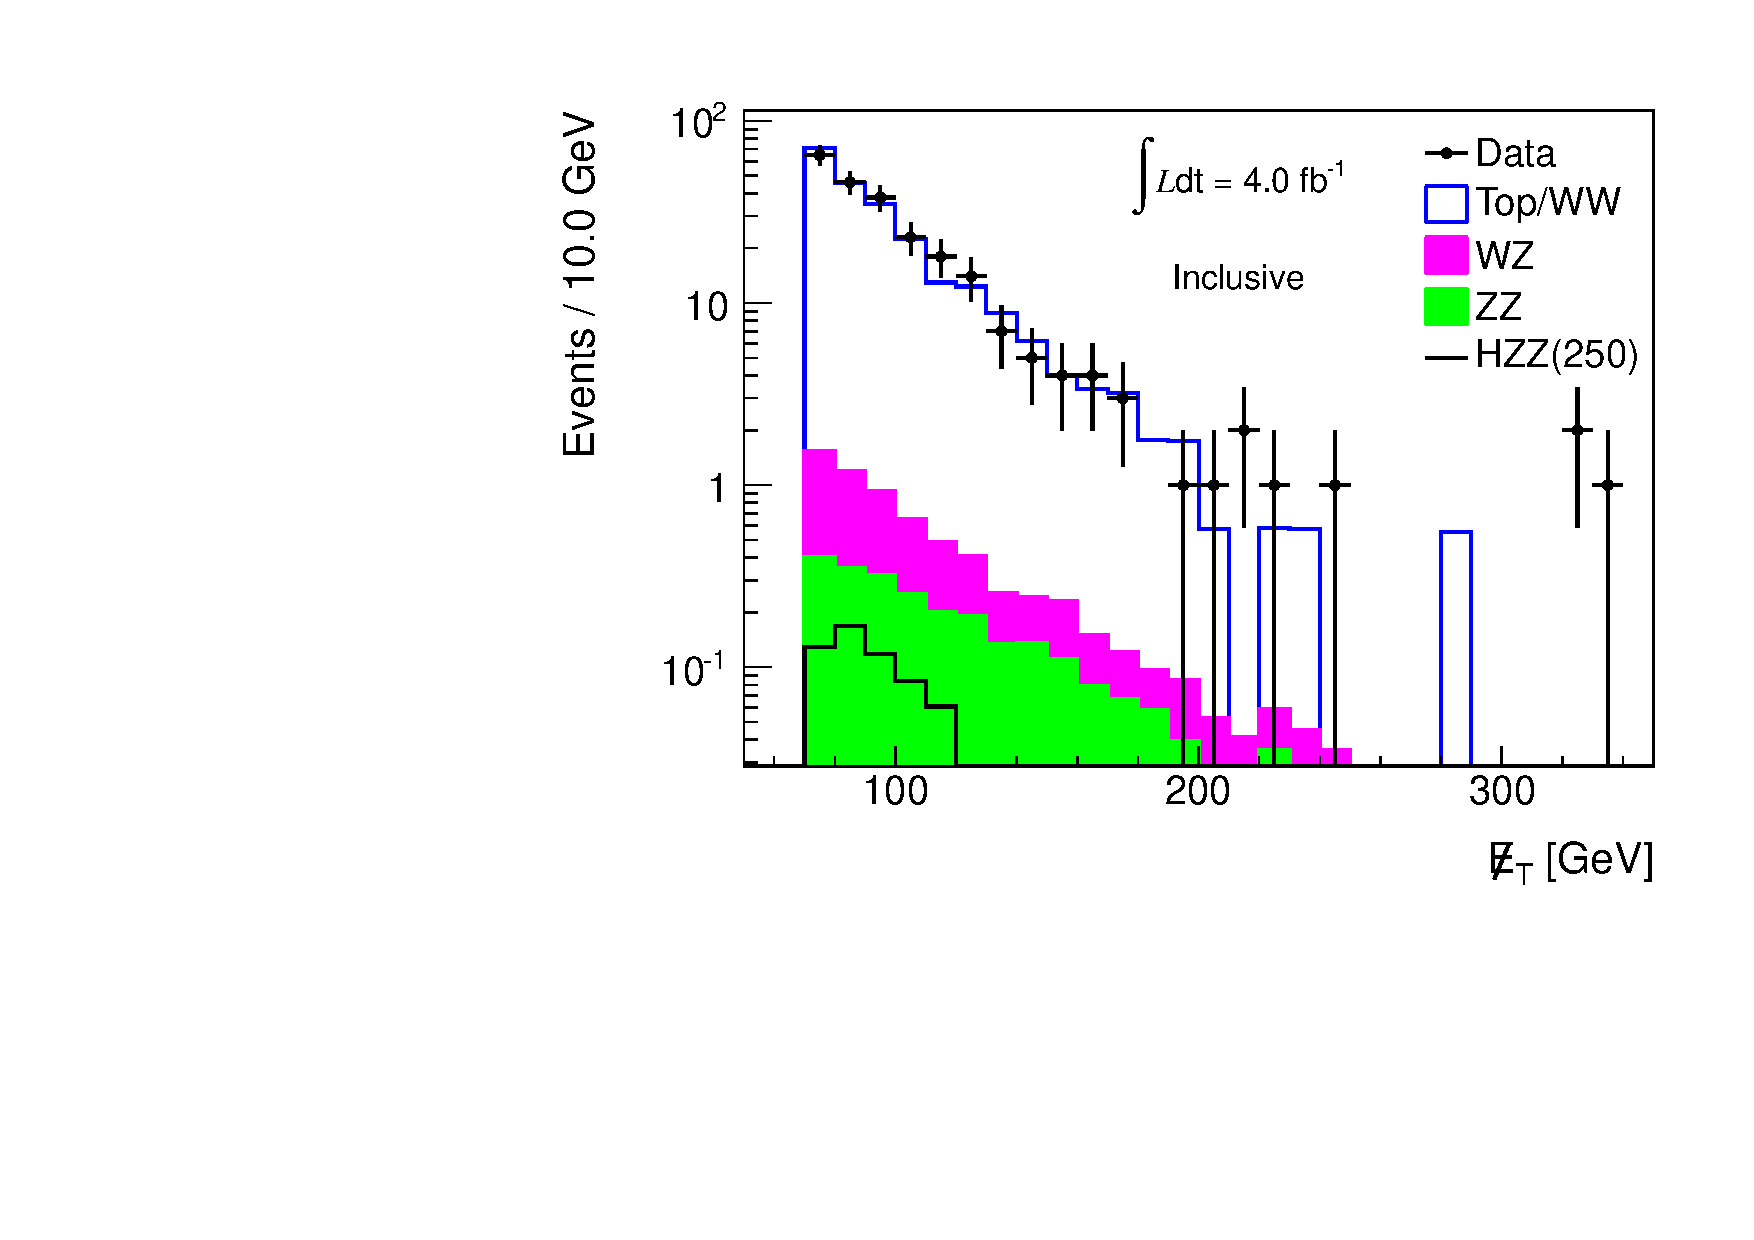
\includegraphics[width=.4\textwidth]{figures/topww_mH250_mm_metlog_incl.pdf}}
\subfigure[Electron channel]{\label{subfig:topww_metlog_ee}
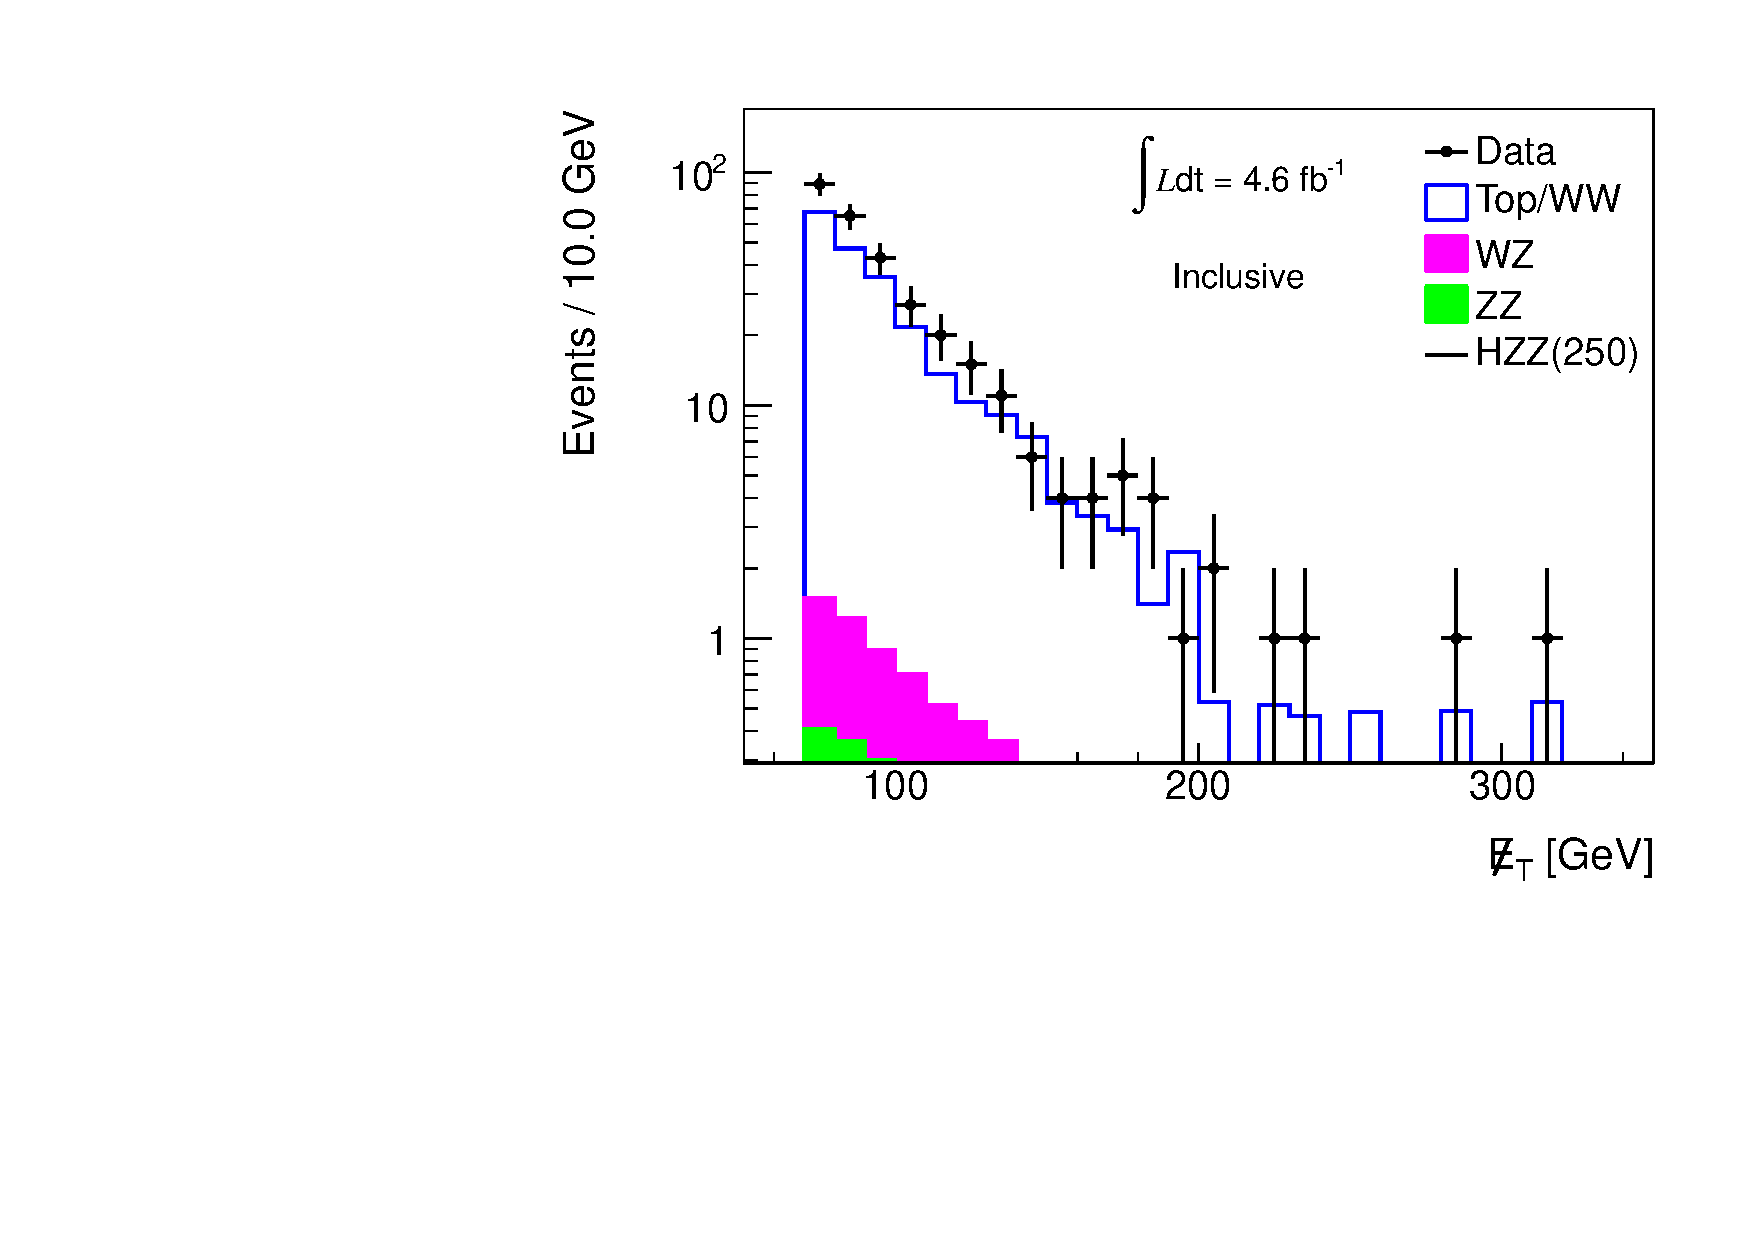
\includegraphics[width=.4\textwidth]{figures/topww_mH250_ee_metlog_incl.pdf}}
\caption{Distribution for the MET in the top/$WW$ control region corresponding 
to $4.0$~\ifb of data in the muon~\subref{subfig:npv_mm} and electron~\subref{subfig:npv_ee} channels, 
compared to the expected from simulation for signal and background. The MC backgrounds are scaled as 
appropriate and the opposite flavor dilepton estimate of the top and $WW$ background is added to the stack.}
\label{fig:topww_metlog}
\end{center}
\end{figure}
%%%%%%%%

%%%%%%%%
\begin{figure}[!hbtp]
\begin{center}
\subfigure[Muon channel]{\label{subfig:topww_mt_mm}
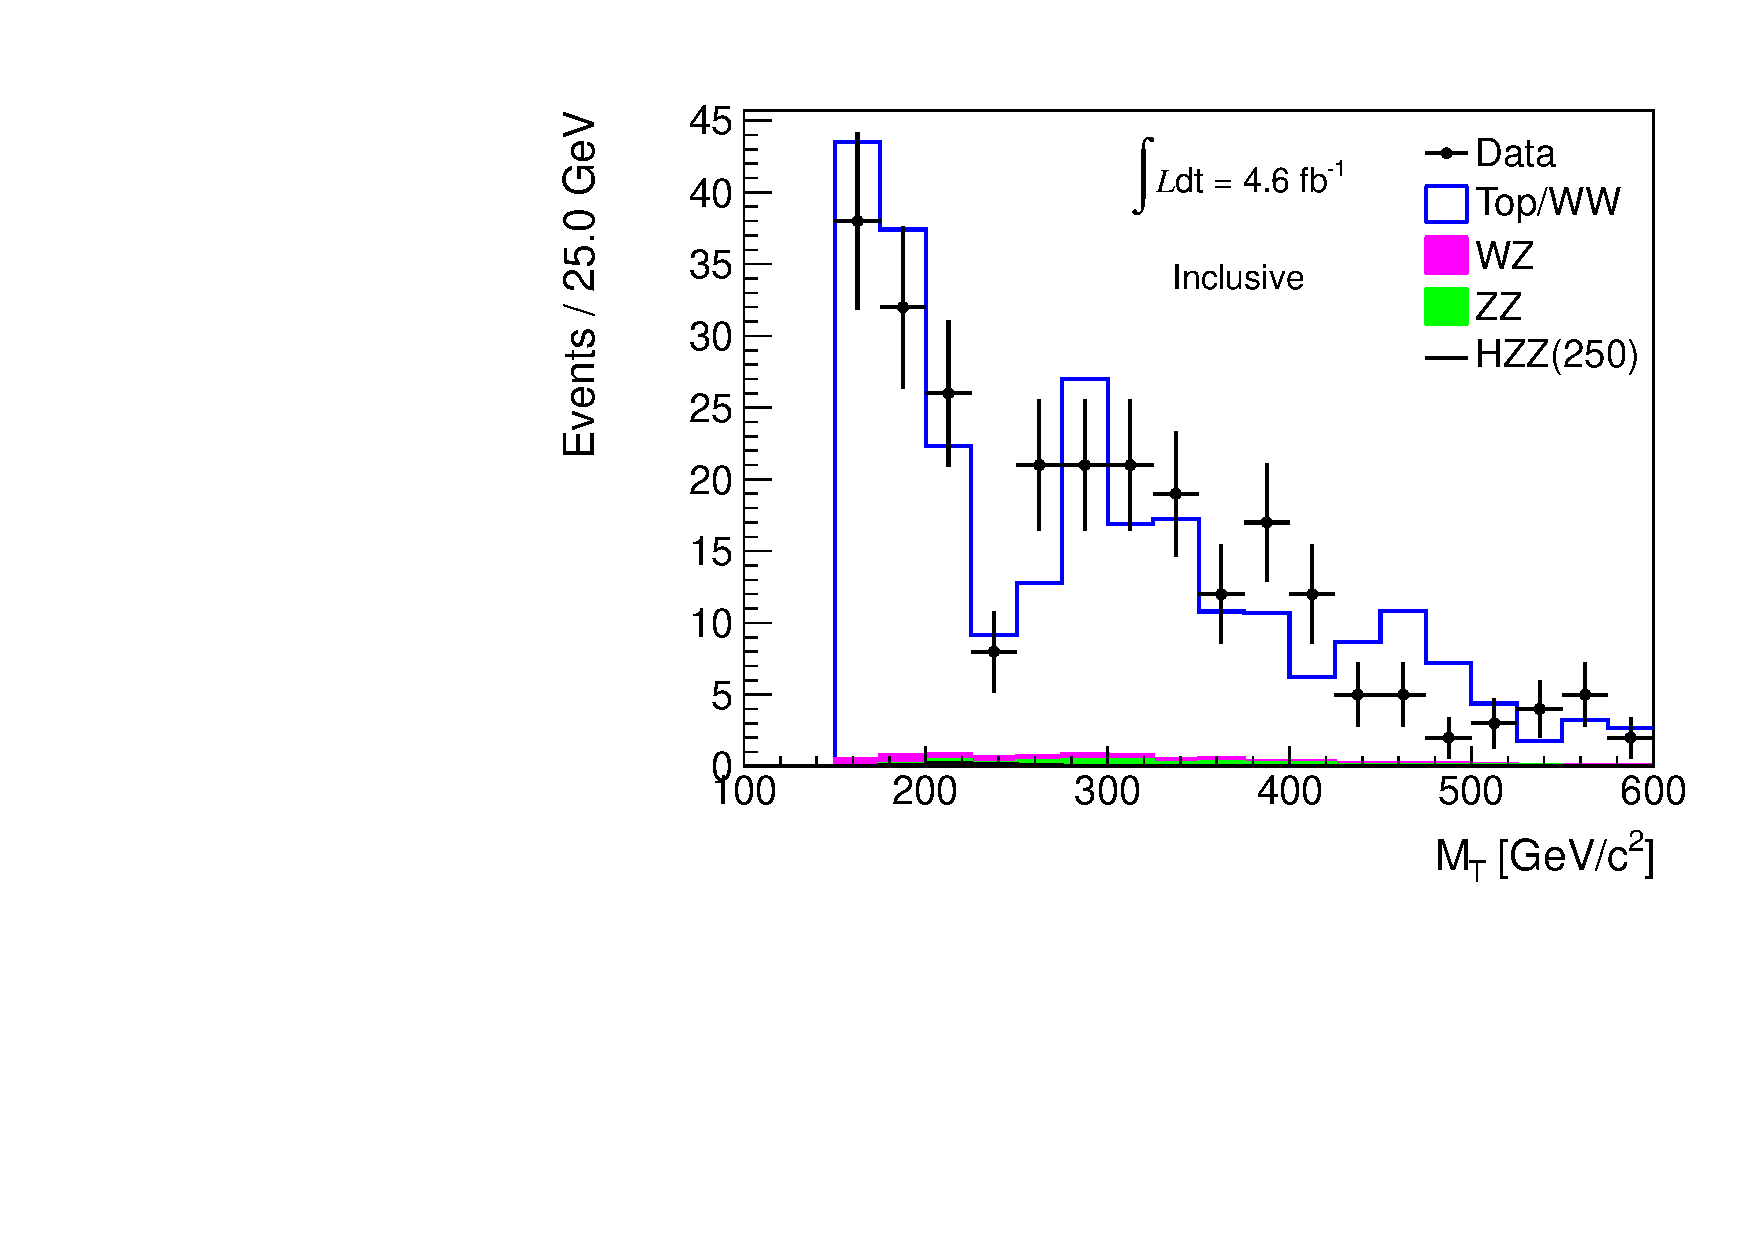
\includegraphics[width=.4\textwidth]{figures/topww_mH250_mm_mt_incl.pdf}}
\subfigure[Electron channel]{\label{subfig:topww_mt_ee}
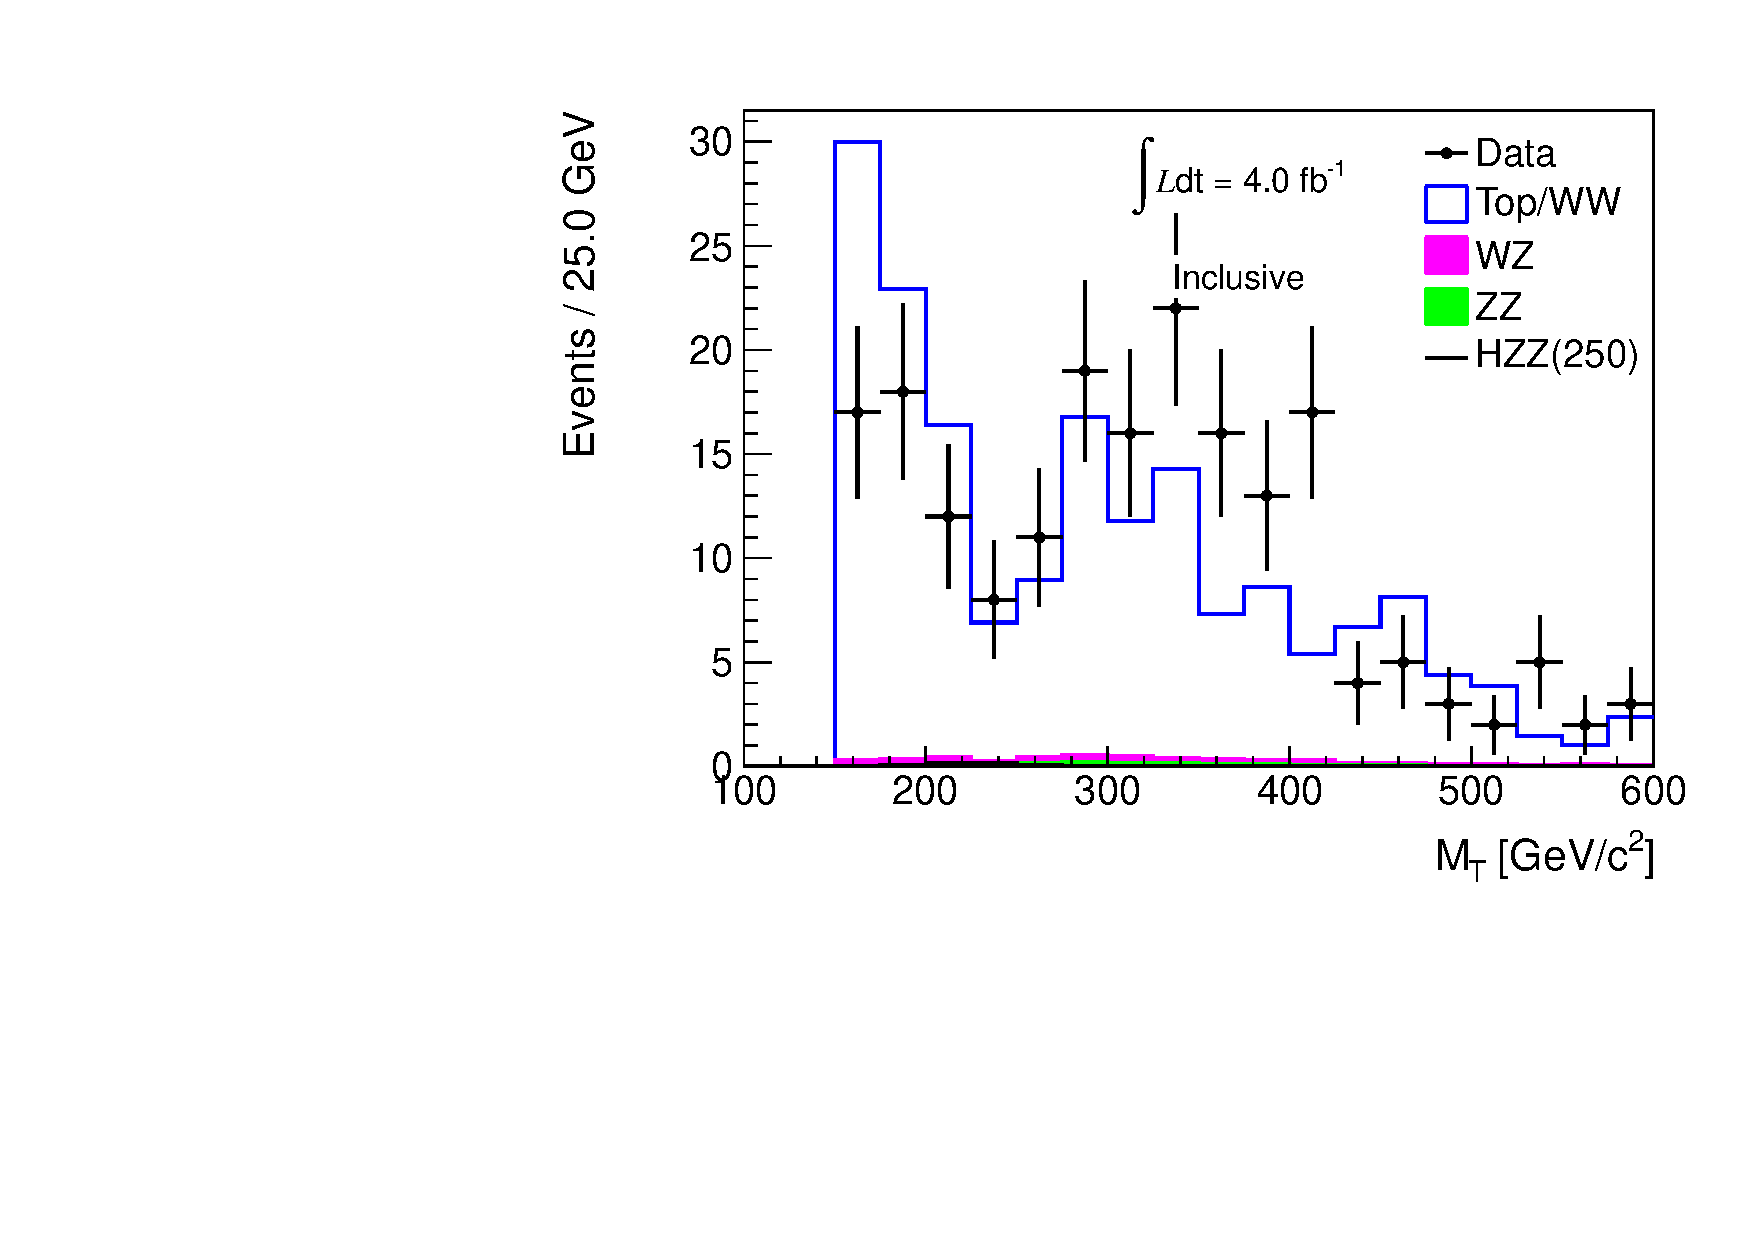
\includegraphics[width=.4\textwidth]{figures/topww_mH250_ee_mt_incl.pdf}}
\caption{Distribution for the dilepton mt in the top/$WW$ control region corresponding 
to $4.0$~\ifb of data in the muon~\subref{subfig:npv_mm} and electron~\subref{subfig:npv_ee} channels, 
compared to the expected from simulation for signal and background. The MC backgrounds are scaled as 
appropriate and the opposite flavor dilepton estimate of the top and $WW$ background is added to the stack.}
\label{fig:topww_mt}
\end{center}
\end{figure}
%%%%%%%%

%%%%%%%%
\begin{figure}[!hbtp]
\begin{center}
\subfigure[Muon channel]{\label{subfig:topww_dphijetmet_mm}
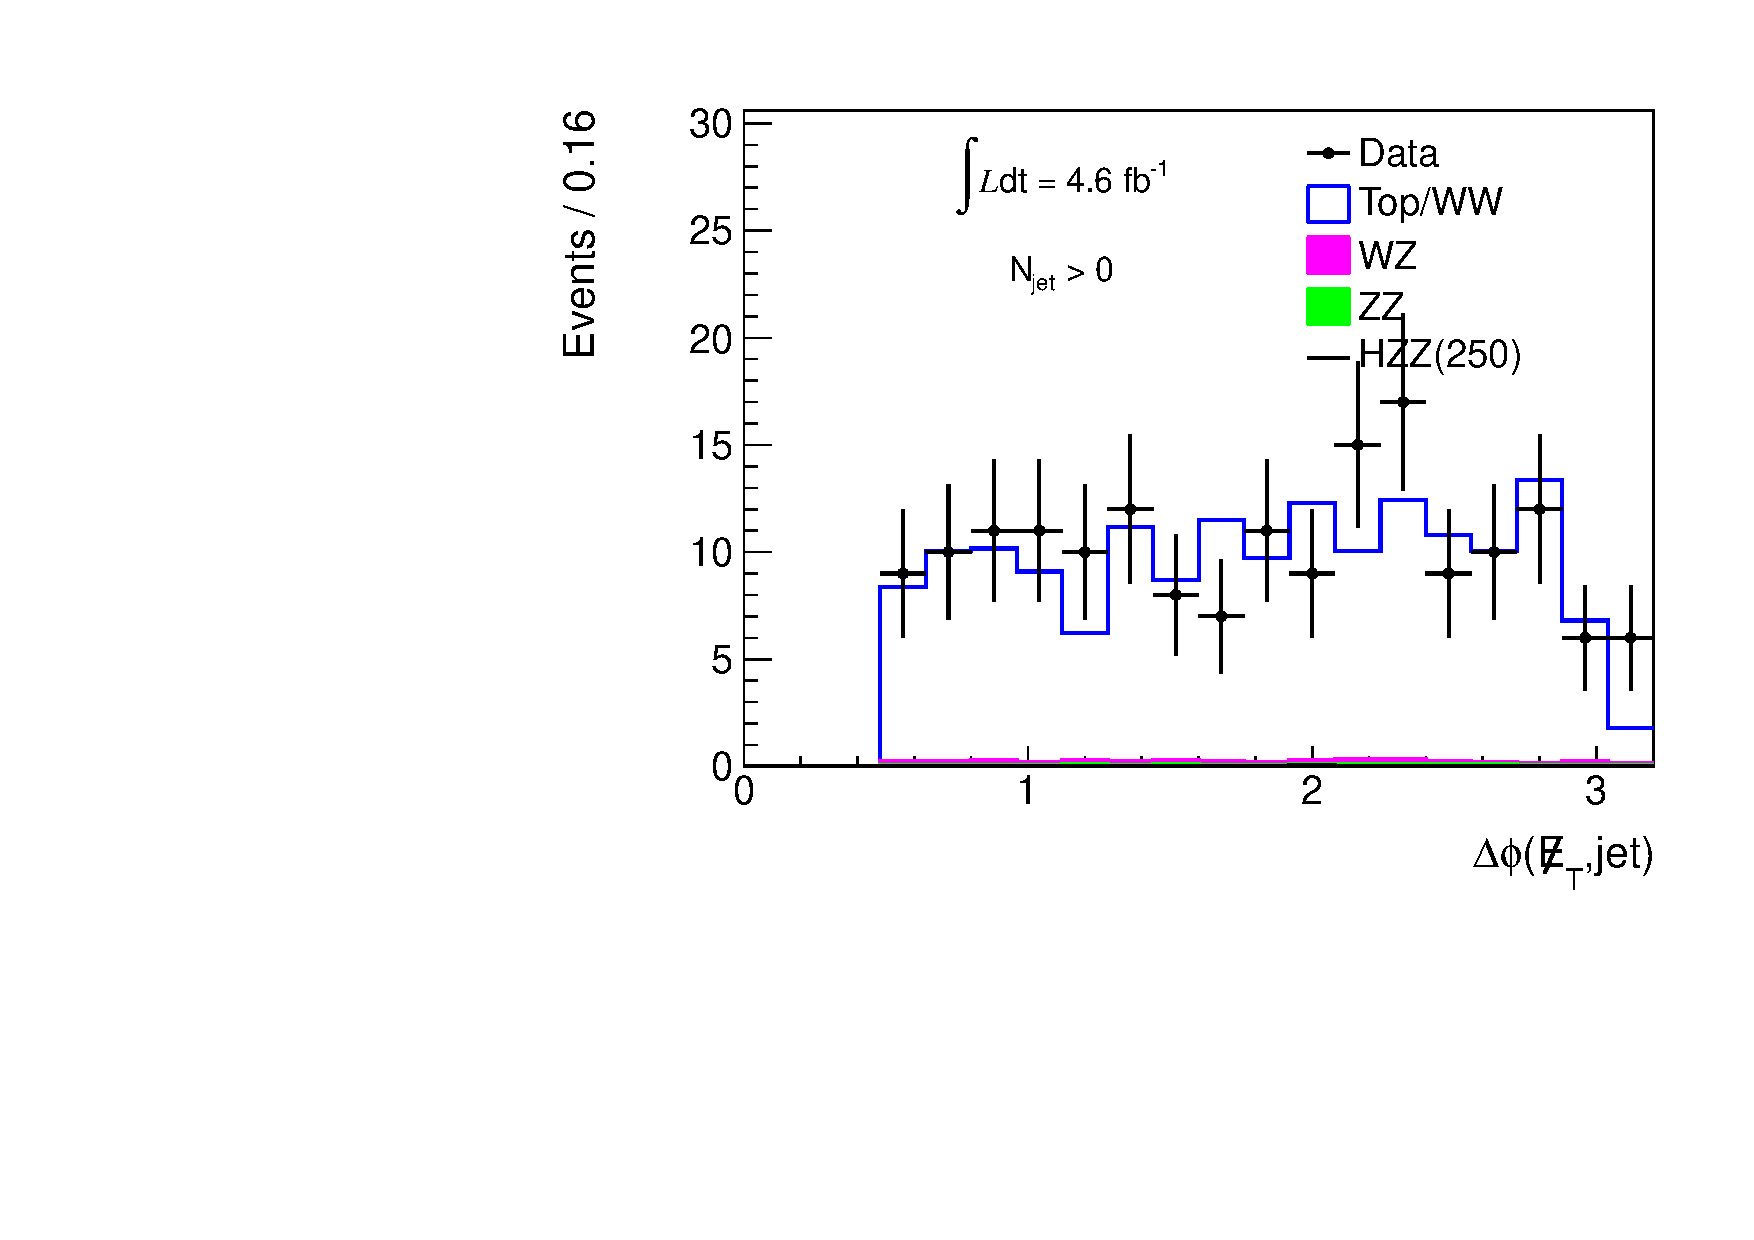
\includegraphics[width=.4\textwidth]{figures/topww_mH250_mm_dphijetmet_incl.pdf}}
\subfigure[Electron channel]{\label{subfig:topww_dphijetmet_ee}
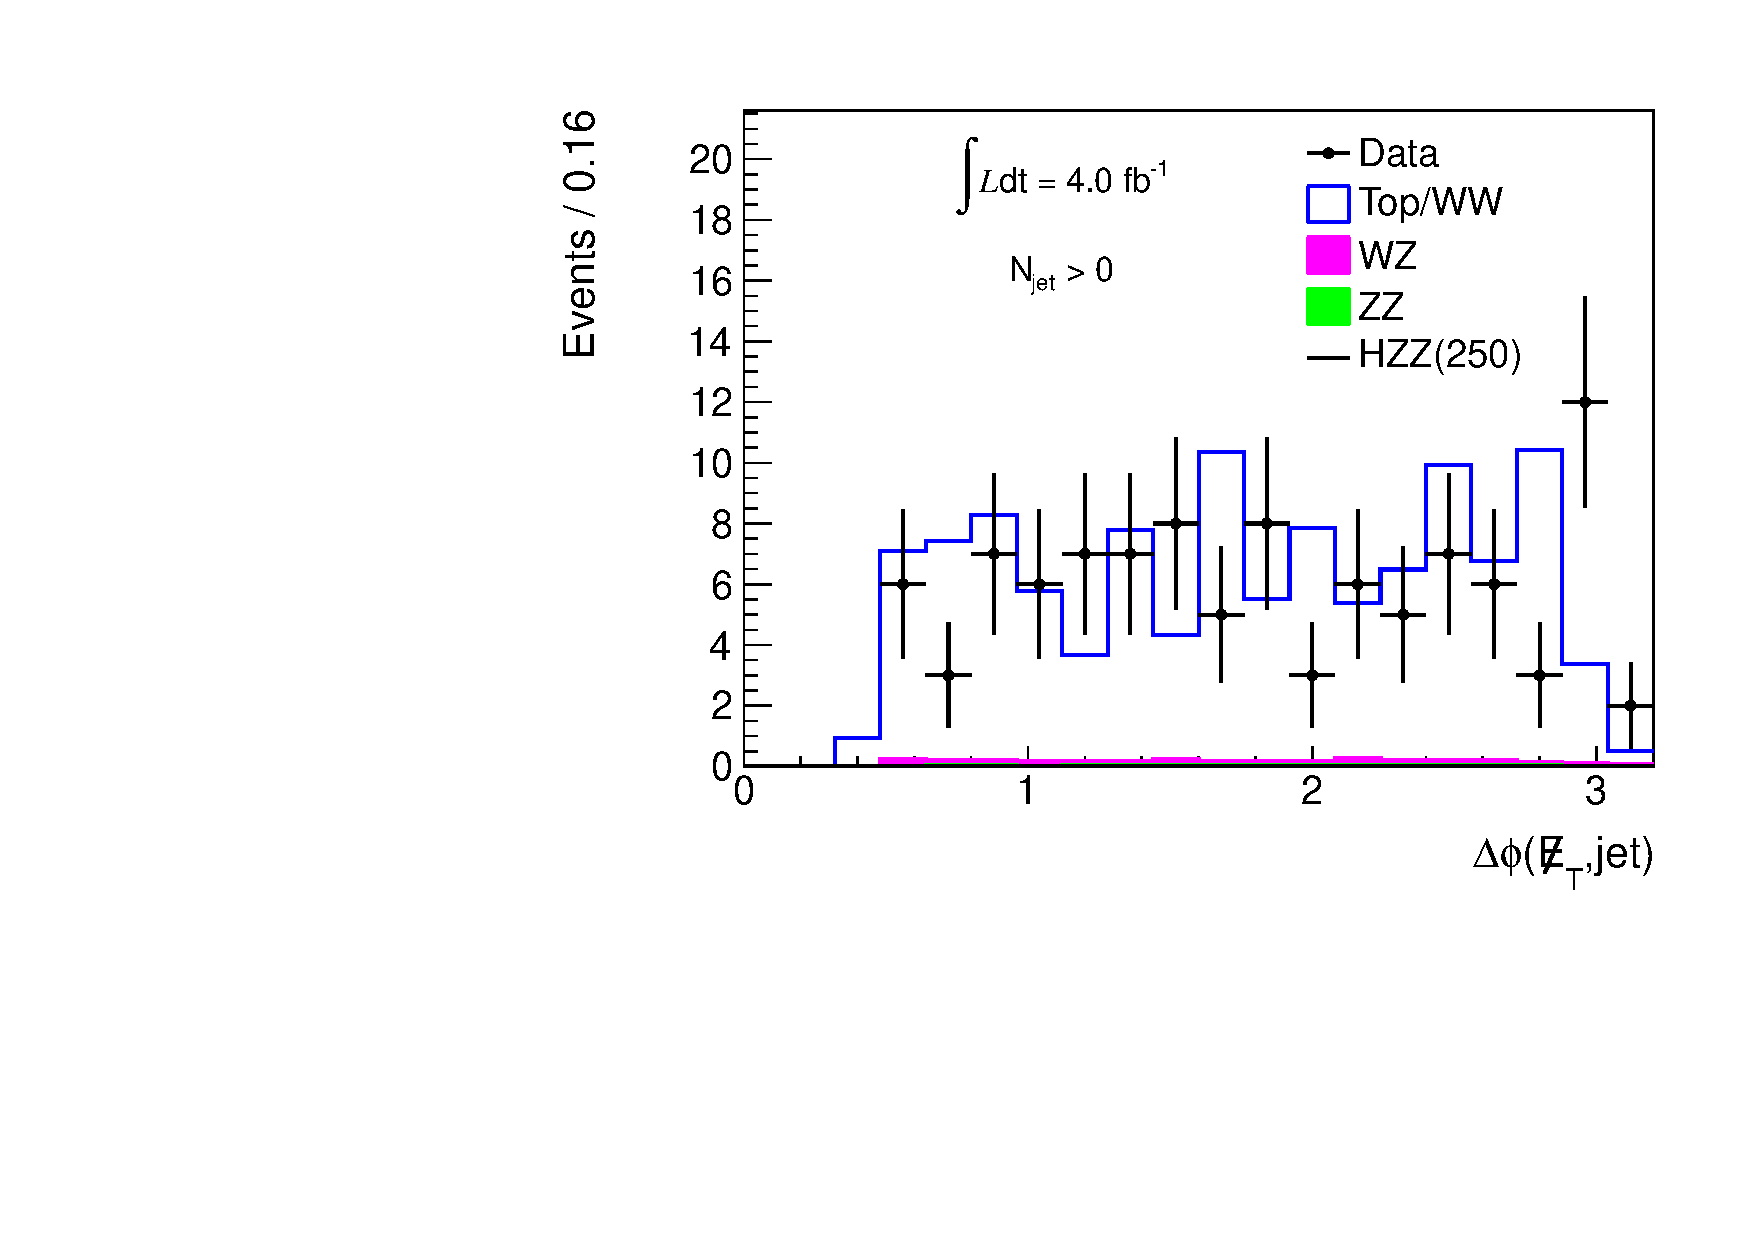
\includegraphics[width=.4\textwidth]{figures/topww_mH250_ee_dphijetmet_incl.pdf}}
\caption{Distribution for the dilepton $\Delta\phi\left(\mbox{jet},\mbox{MET}\right)$ in the top/$WW$ control region corresponding 
to $4.0$~\ifb of data in the muon~\subref{subfig:npv_mm} and electron~\subref{subfig:npv_ee} channels, 
compared to the expected from simulation for signal and background. The MC backgrounds are scaled as 
appropriate and the opposite flavor dilepton estimate of the top and $WW$ background is added to the stack.}
\label{fig:topww_dphijetmet}
\end{center}
\end{figure}
%%%%%%%%
